\documentclass[final,fmstyle]{./util/ucathesis}
% La opcion 'final' muestra los graficos, para generar una version sin los graficos utiliza la opcion 'draft'

% paquetes recomendados
%\usepackage[chapter]{theorems}
%\usepackage{symbols}
%\usepackage{url}
\usepackage{amsmath,amsthm}

\usepackage[T1]{fontenc}
\usepackage[spanish]{babel}
\usepackage[utf8]{inputenc}
\usepackage{csquotes}
\usepackage[style=numeric,sorting=none,backend=biber]{biblatex}
\usepackage{listings}
\addbibresource{referencias.bib}


% custom commands
\newcommand{\foreign}[1]{{\it #1}}
\DeclareMathOperator*{\argmax}{arg\,max}
\algsetup{indent=2em}

% \setcounter{tocdepth}{3}

\begin{document}
\lstset{
    language=java,
    basicstyle=\small\sffamily,
    numbers=left,
    numberstyle=\tiny,
    frame=tb,
    columns=fullflexible,
    showstringspaces=false
}


% incluye aqui los capitulos (un archivo .tex por capitulo)

\chapter{Estado del Arte de los sistemas información georeferenciada}
\chapter{Dengue en Paraguay}

\section{Ciclo biológico del Aedes aegypti}
\label{sec:caracteristicas-biologicas}
De todas las especies de mosquitos conocidos, con importancia en salud pública, la Aedes aegypti,
es considerada la más peligrosa por tener la capacidad de transmitir el mayor número de enfermedades arbovirales\footnote{Las infecciones arbovirales son los virus que se transmiten por
los mosquitos. \textit{Arbo} es una abreviatura que significa transmitida por los artrópodos, los
cuales son insectos.}, al hombre \cite{ThironIzcazaJ2003}.

Los sitios de cría del Aedes aegypti son fundamentalmente artificiales: urbanos (en baldíos,
cementerios, desarmaderos, basurales) o domésticos (neumáticos, floreros, botellas, bebederos de
animales, latas abiertas o contenedores de cualquier tipo, cisternas, vasijas, tinajas, todo tipo
de recipientes en desuso, aun pequeños, prácticamente de cualquier objeto que retenga agua)
\cite{world2009dengue, directricesDetvArg}.

\begin{figure}[!htbp]
\centering
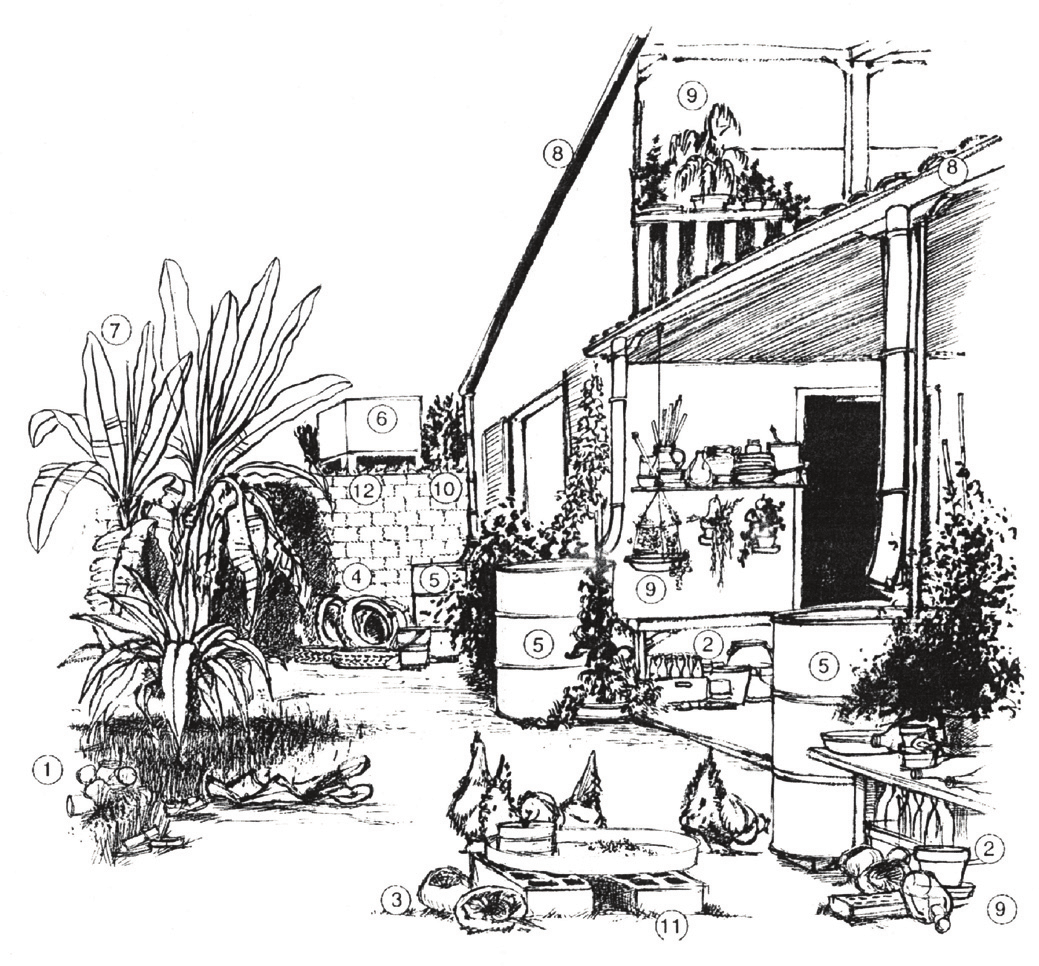
\includegraphics[width=0.8\textwidth]{capitulo-3/graphics/criaderos-domicilio.png}
\caption{\label{fig:cap3-larvitrampas} Ejemplo de los posibles lugares de cría del mosquito Aedes
aegypti, en los alrededores de la casa (Tomado de \cite{manualControlArg2009}).}
\end{figure}


Prefieren agua limpia, con bajo tenor orgánico y de sales disueltas. La puesta de huevos la
realizan en la superficie del recipiente. Algunos recipientes le son más atractivos que otros, en
especial los de color oscuro, de boca ancha, que están al nivel del suelo y se encuentran en la
sombra \cite{ThironIzcazaJ2003}.

Su ciclo de vida manifiesta una metamorfosis completa, es decir que las formas inmaduras salidas
del huevo son completamente diferentes al adulto, las primeras son de vida acuática, las segundas
de vida aérea \cite{directricesDetvArg}, donde su desarrollo se encuentra dividido en cuatro
etapas, huevo, larva, pupa y adulto \cite{web-site:gMonteroBiologia}
(\figref{fig:cap3-ciclo-de-vida}).

\begin{figure}[!htbp]
\centering
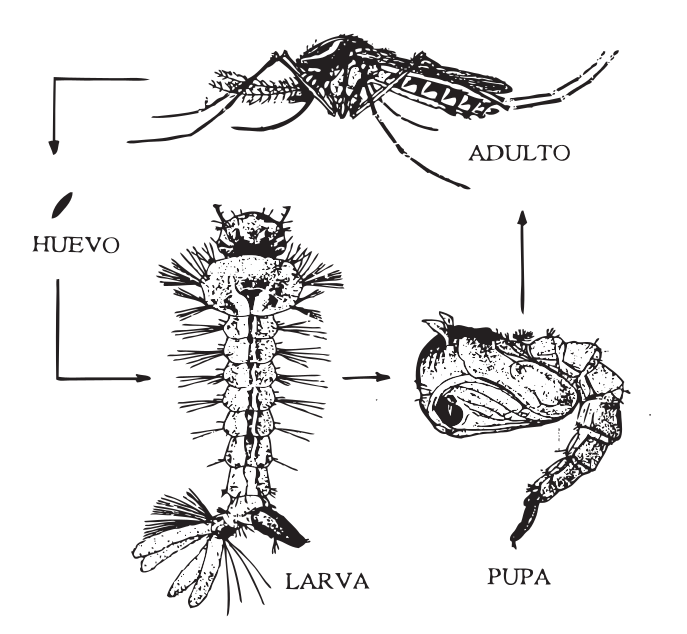
\includegraphics[width=0.7\textwidth]{capitulo-3/graphics/ciclo-de-vida.png}
\caption{\label{fig:cap3-ciclo-de-vida} Ciclo de vida del Aedes aegypti (Tomado de
\cite{directricesDetvArg}).}
\end{figure}

\subsection{Huevo}
\label{subsec:ciclo-biologico-huevo}
Los huevos miden aproximadamente un milímetro de longitud, son depositados uno a uno al ras del agua quedando adheridos a las paredes del recipiente \cite{ThironIzcazaJ2003}. Cada vez que sube el
nivel del agua en el recipiente eclosiona un grupo de huevos, de este modo, se aseguran una
eclosión escalonada que permite la supervivencia aún en condiciones desfavorables
\cite{directricesDetvArg}.

\begin{figure}[!htbp]
\centering
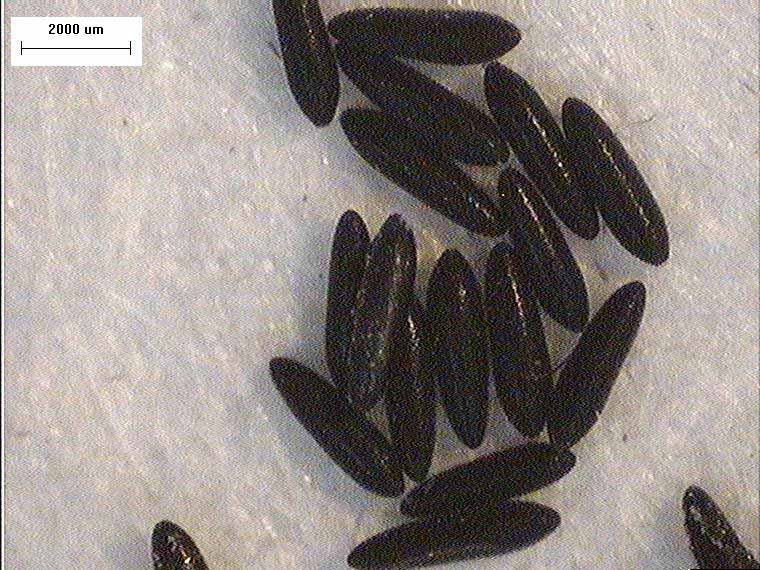
\includegraphics[width=0.5\textwidth]{capitulo-3/graphics/huevos.png}
\caption{\label{fig:cap3-huevos} Huevos del mosquito Aedes aegypti (Tomado de
\cite{sivanathan2006ecology}).}
\end{figure}

Al momento de la postura son de coloración blanca, casi transparentes, en contacto con el aire van
adoptando la coloración oscura característica \cite{directricesDetvArg} (\figref{fig:cap3-huevos}).
La fecundación ocurre al momento de la postura del huevo, en donde el desarrollo embrionario
transcurre en alrededor de 48 horas si el ambiente es húmedo y cálido, si la temperatura es baja
se prolonga hasta por cinco días \cite{ThironIzcazaJ2003}. Los huevos son formas de resistencia que
pueden sobrevivir durante muchos meses en clima adverso hasta que las condiciones ambientales
favorezcan su eclosión \cite{directricesDetvArg}.

\subsection{Larva}
\label{subsec:ciclo-biologico-larva}
Los huevos eclosionan dando lugar a formas larvarias, acuáticas, nadadoras, de respiración aérea
\cite{directricesDetvArg} y es el período de mayor alimentación y crecimiento
\cite{web-site:gMonteroBiologia}. Pasan la mayor parte del tiempo alimentándose del material
orgánico sumergido o acumulado en las paredes y el fondo del recipiente
\cite{web-site:gMonteroBiologia, directricesDetvArg}.

Las larvas que emergen inician un ciclo de 4 estadios larvales \cite{web-site:gMonteroBiologia},
donde, estos estadios definen su período de crecimiento y desarrollo \cite{ThironIzcazaJ2003}. El
primer estadio larval es la forma que emerge del huevo, con una duración de uno a dos días. Este
periodo esta dedicado a la alimentación y el crecimiento, posteriormente ocurre la muda y surge el
segundo estadio \cite{ThironIzcazaJ2003}. En el segundo estadio, la cápsula cefálica y el sifón
son blandos y transparentes, al extenderse permite el subsecuente desarrollo, se endurecen y
oscurecen \cite{ThironIzcazaJ2003}. Después del segundo estadio, la cápsula cefálica y el sifón no
cambian de tamaño, el tórax y el abdomen crecen considerablemente durante cada fase
\cite{ThironIzcazaJ2003}.

\begin{figure}[!htbp]
\centering
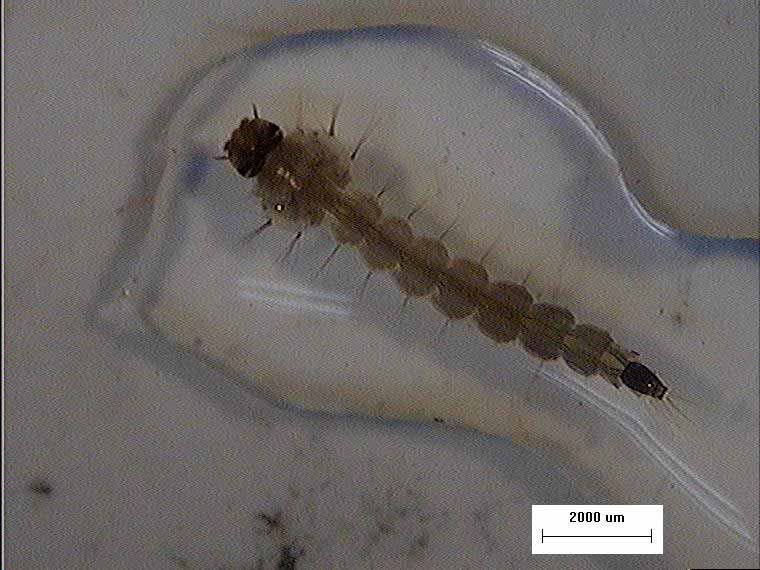
\includegraphics[width=0.5\textwidth]{capitulo-3/graphics/larva.png}
\caption{\label{fig:cap3-larvas} Larva del mosquito Aedes aegypti (Tomado de
\cite{sivanathan2006ecology}).}
\end{figure}

La duración del desarrollo larval está en función de la temperatura, la disponibilidad de alimento
y la densidad de larvas en el criadero \cite{ThironIzcazaJ2003}. Los primeros tres estadios se
desarrollan rápidamente, mientras que el cuarto toma más tiempo, debido a que aumenta
considerablemente su tamaño y peso \cite{ThironIzcazaJ2003, web-site:gMonteroBiologia},
en condiciones de baja temperatura o escasez de alimento el cuarto estadio puede prolongarse por
varias semanas \cite{ThironIzcazaJ2003}. En condiciones óptimas, el período larval desde la
eclosión hasta la pupación puede ser de cinco días, pero por lo regular ocurre de siete a catorce
días \cite{ThironIzcazaJ2003}.

La mortalidad, más elevada ocurre frecuentemente en los primeros estadios larvales
\cite{ThironIzcazaJ2003}, donde la principal causa es atribuida a la inestablididad de los
criaderos que sirven como habitad.

\subsection{Pupa}
\label{subsec:ciclo-biologico-pupa}
Las pupas, al igual que las larvas, son acuáticas, estas no se alimentan, su función es la
metamorfosis del estadio larval al adulto \cite{ThironIzcazaJ2003}. El período pupal dura de 1
a 3 días en condiciones favorables, con temperaturas entre 28 y 32 \textcelsius
\cite{web-site:gMonteroBiologia}, emergiendo alrededor del 88\% de los adultos en cuestión de 48
horas \cite{ThironIzcazaJ2003}. Las variaciones extremas de temperatura pueden dilatar este período
\cite{web-site:gMonteroBiologia}.

\begin{figure}[!htbp]
\centering
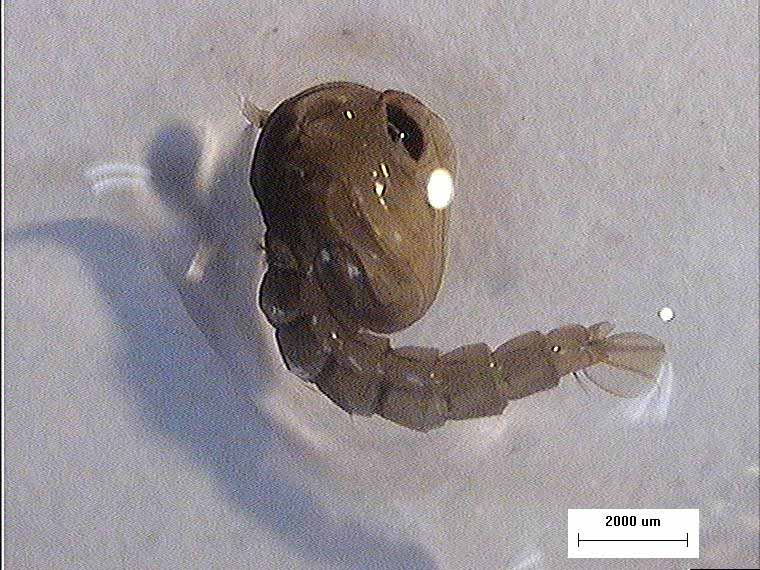
\includegraphics[width=0.5\textwidth]{capitulo-3/graphics/pupa.png}
\caption{\label{fig:cap3-larvas} Larva del mosquito Aedes aegypti (Tomado de
\cite{sivanathan2006ecology}).}
\end{figure}

\subsection{Adulto}
\label{subsec:ciclo-biologico-adulto}
La función más importante del adulto es la reproducción \cite{ThironIzcazaJ2003}. Aproximadamente
la mitad de los adultos emergentes son hembras \cite{otero2006stochastic, manrique1998desarrollo}.
Los adultos recién emergidos permanecen las primeras 24 horas en fase teneral\footnote{Período en
que el insecto adulto está recién salió de la envoltura pupal o piel de ninfa.}, tiempo en que se
efectúa el endurecimiento y oscurecimiento de su cutícula \cite{luevano1993ciclo}. Pueden
permanecer vivos en el laboratorio durante meses y en la naturaleza pocas semanas, con una
mortalidad diaria de 10\%, la mitad de los mosquitos morirán durante la primera semana y 95\% en
el primer mes \cite{ThironIzcazaJ2003}.

\begin{figure}[!htbp]
\centering
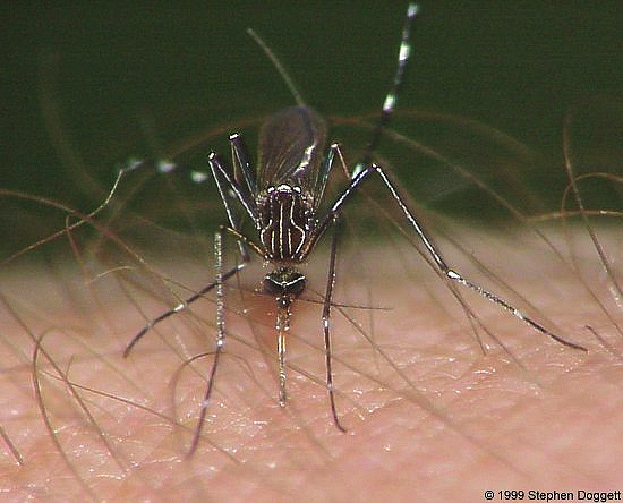
\includegraphics[width=0.5\textwidth]{capitulo-3/graphics/adulto.png}
\caption{\label{fig:cap3-larvas} Adulto del mosquito Aedes aegypti (Tomado de
\cite{directricesDetvArg}).}
\end{figure}

Las partes bucales del macho no están adaptadas para chupar sangre, se alimentan de carbohidratos
de cualquier fuente accesible como frutos o néctar de flores que satisface sus requerimientos
energéticos \cite{ThironIzcazaJ2003}. Las hembras también se alimentan de esta misma fuente como
complemento indispensable, sin embargo necesitan alimentarse de sangre para obtener las proteínas
necesarias para la formación de los huevos \cite{ThironIzcazaJ2003}.

Antes de 24 horas ambos sexos están listos para el apareamiento, alrededor del 58\% de las hembras
nulíparas \footnote{Nulíparas son aquellas hembras jóvenes que no han ovipuesto.} son inseminadas
antes de su primera alimentación sanguínea, un 17\% durante y el 25\% es inseminada entre la
segunda alimentación y la primera oviposición \cite{ThironIzcazaJ2003}. Una inseminación es
suficiente para fecundar todos los huevos que la hembra produzca en toda su vida
\cite{ThironIzcazaJ2003}. El apareamiento, que por lo general se efectúa durante el vuelo, es
debido a que el macho es atraído por el sonido emitido por las alas de la hembra
\cite{ThironIzcazaJ2003}. El patrón diario de alimentación de los mosquitos, varia de acuerdo a
las localidades y subespecies\cite{luevano1993ciclo}.

Los mosquitos tienen la particularidad de volar en sentido contrario a la dirección al viento
\cite{ThironIzcazaJ2003, web-site:speedAnimals} a una velocidad máxima de dos kilómetros por hora
\cite{web-site:speedAnimals,kaufmann2004flight}. Por sus hábitos, es considerado como doméstico
\cite{luevano1993ciclo}, tiende a permanecer en el lugar en donde emergió
\cite{cabezas2005dengue,ThironIzcazaJ2003}, siempre y cuando no exista algún factor que la
perturbe o no disponga de huéspedes, sitios de reposo y de postura  \cite{ThironIzcazaJ2003}. Por
lo general el mosquito no sobrepasa los 50 a 100 metros durante su vida \cite{cabezas2005dengue}.
Los sitios de cría del Aedes aegypti son fundamentalmente artificiales o domésticos
\cite{directricesDetvArg}. En caso de no haber recipientes adecuados, la hembra grávida es capaz
de volar hasta tres kilómetros en busca de este sitio \cite{ThironIzcazaJ2003}.

Es común que después de cada alimentación sanguínea la hembra desarrolle un lote de huevos, la
cantidad de huevos depende de la alimentación que puede variar entre 100 a 200 huevos
\cite{cabezas2005dengue}. El intervalo de tiempo que transcurre entre la alimentación sanguínea y
la postura, denominado ciclo gonotrófico, es de 48 horas en los trópicos bajo condiciones óptimas
de temperatura\cite{ThironIzcazaJ2003}. Dentro de la bionomía de vectores, una fase muy importante
es el ciclo gonotrófico, el cual es un proceso fisiológico que consiste en la digestión de la
comida sanguínea y desarrollo de los ovarios \cite{luevano1993ciclo}.

%%!TEX root = ../tesis.tex
\chapter{Definici\'on del Problema}
\label{sec:problema}

deficion general del problema

% introduccion

%~ problema general
%~ problema especifico
%~ problema motivacion

%%!TEX root = ../tesis.tex
\chapter{Soluci\'on Propuesta}
\label{sec:solucion}

% introduccion
soluci\'on propuesta...


%!TEX root = ../tesis.tex
\section{Descripci\'on General}
\label{sec:solucion-general}


%!TEX root = ../tesis.tex
\section{Identificación de los focos de dengue}
\label{sec:solucion-instantanea}
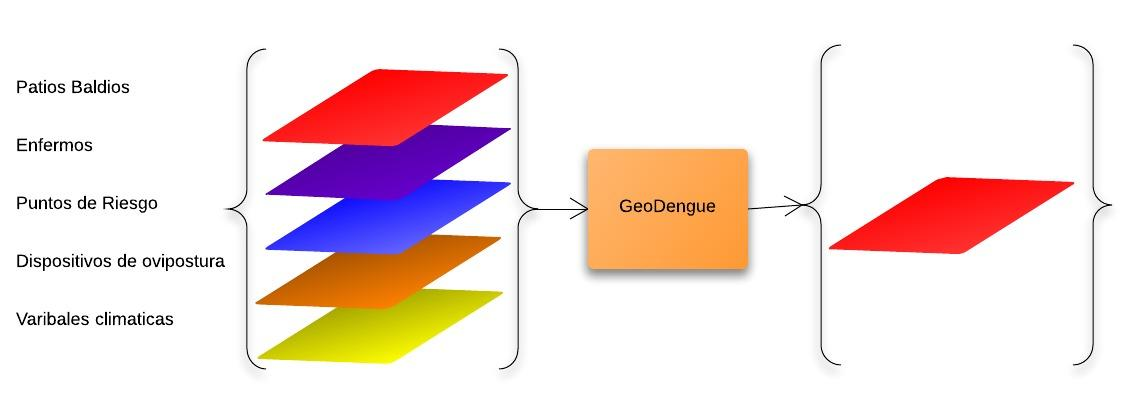
\includegraphics[ scale=0.35]{./graphics/modelo-base.jpeg}

Mediante técnicas de interpolación espacial los datos de entrada serán procesados y representados en la zona de estudio como polígonos que representan focos de la enfermedad.

Los focos se determina según los valores conocidos de las larvitrampas mediante interpolación, esto representa un instante \cite{AnusuyaSpeech20097}.

%!TEX root = ../tesis.tex
\section{Proceso Evolutivo}
\label{sec:solucion-evolutivo}
El proceso de evolución de las muestras consiste en un proceso, en el cual las muestras obtenidas mediante los dispositivos de ovipostura  son expuestas a un conjunto de variaciones en un periodo de tiempo. Las variaciones que, principalmente, afectan a las muestras son :

\begin{itemize}
    \item \em Las variaciones del clima en dicho periodo \rm: Se someten las muestras obtenidas a las distintas variaciones climáticas ocurridas en el periodo de tiempo seleccionado para el estudio.
    \item \em La naturaleza del mosquito \rm: Cada elemento de la muestra, es sometido a cambios considerando la naturaleza del mosquito. Los aspectos que se tienen en cuenta son su ciclo de vida del mosquito, ciclo reproductivo y el desplazamiento.
\end{itemize}
Todo lo que tenga que ver con un análisis evolutivo(proyección) en un periodo de tiempo, se va tratar diferente. Se va tener en cuenta las variaciones del clima en dicho periodo. se debe hacer evolucionar las larvitrampas por cada día del periodo estudiado.

\subsection{Afirmaciones}

\begin{itemize}
    \item La población contiene a todos los mosquitos (macho, hembra) en cualquiera de sus estados(huevo,larvas, pupa, adulto).
    \item La población inicial está compuesta por el conjunto de mediciones de los dispositivos de ovipostura.
    \item La salida final a interpolar van a ser larvas, salida complementaria es el resto de la población.
    \item Un mosquito de la población tiene los siguientes atributos :
        \begin{itemize}
            \item Sexo : Macho o hembra
            \item Edad : cantidad de días que lleva vivo el mosquito.
            \item Estado : Huevo, Larva, Pupa, Adulto..
            \item Ubicación : coordenadas longitud y latitud
            \item Dispositivo de origen : el código del dispositivo de ovipostura de origen.
            \item Expectativa de vida : es un valor numérico que varía de acuerdo a las condiciones climáticas a las que es sometido el mosquito.
        \end{itemize}
   \item Periodo es el intervalo de tiempo al que será sometido la población inicial a evolución.
\end{itemize}


\subsection{Descripción de los pasos del pseudo código (ver tabla)}

1- Se itera sobre cada día contemplado dentro del periodo de estudio.
De dichos días se conocen distintas propiedas como la temperatura máxima,
media, y mínima. Además se conoce el nivel de humedad y si hubo o no
lluvias.

2- Se procesa cada mosquito dentro de la población. La población está
compuesta por el total de mosquitos registrados mediante el conteo de
larvitrampas.

3- A cada mosquito de la poblacion se le hace desarrollar en el día.
En otras palabras; aplicar las condiciones del día actual al mosquito. Dicho
proceso funciona como modelo de simulación de la vida de un mosquito
dada las condiciones del día actual. Para poder realizar
correctamente el proceso evolutivo es necesario tener en cuenta la
ubicación del mosquito, su estado actual (en que fase de desarrollo se
encuentra y cual es su espectativa de sobrevivencia) y su tiempo de vida
(edad actual).

4- En este paso se verifica si la expectativa de vida del mosquito ha
disminuido a 0. Lo que implica que el mosquito está muerto sea cual sea
su estado. Esto puede darse en un día muy frío o muy caluroso o por un proceso
selección natural.

5- En el caso de que el mosquito haya muerto se lo excluye de la
población de estudio

6- En caso contrario, se establece una serie de heurísticas de reproducción
para dar lugar a nuevos individuos. En el caso de que en la población exista
al menos 1 hembra y 1 macho adulto en proximidad. Datos sobre la tendencia
de ovipostura y cantidad de huevos que una hembra deposita se suman al
análisis para lograr mayor precisión

7- Se realiza una operación que en donde se utilizan variables
georeferenciadas de acuerdo a la posición del mosquito para estimar
la posibilidad de que encuentre criadero fértil para depositar sus huevos

8- Se aplica la operación de poner huevos si se aplica para el mosquito actual

9- Se añaden a la población los nuevos mosquitos. (el valor de la variable
huevos puede ser NULL)



\begin{lstlisting}[caption=Pseudocódigo del proceso evolutivo, label=a_label,  float=t]
for (dia in Periodo) {
    for( mosquito in Poblacion){
        mosquito.desarrollar(dia)
        if(mosquito.es_viejo() or mosquito.esta_muerto()){
            Poblacion.remove(mosquito)
        }else if(mosquito.se_reproduce(dia)){
            mosquito.buscar_criaderos(dia)
            var huevos = mosquito.poner_huevos(dia)
            Poblacion.add(huevos)
        }
    }
}
\end{lstlisting}

%!TEX root = ../tesis.tex
\section{Salidas Esperadas}
\label{sec:solucion-salidas}

El resultado del algoritmo es una población final al final del periodo de estudio
de donde se puede determinar la cantidad de mosquitos hembras adultas y su posición entre otras informaciones.

La cantidad de mosquitos hembras adultas y su posición permiten evaluar el crecimiendo o decrecimiento de la población y georeferenciar los focos \textit{de la enfermedad teniendo en cuenta la densidad poblacional.
Identificación de los focos de dengue}

Mediante los datos de entrada se podrá determinar los distintos focos de la enfermedad y su nivel de gravedad. Mediante técnicas de interpolación espacial los datos de entrada serán procesados y representados en la zona de estudio como polígonos que representan focos de la enfermedad.

\subsection{Correlación de variables}
Analizar la influencia de las variables sobre el resultado final y determinar si existen dependencias entre las mismas. Por ejemplo; analizar la influencia del par de datos de entrada (temperatura, humedad) sobre la formación de un foco de la enfermedad del dengue. Expresar la dependencia de variables, en el caso de existir, mediante un gráfico en función del tiempo para visualizar su comportamiento.

\subsection{Datos estadísticos}
Resúmenes que representan información útil dentro del marco de estudio de la enfermedad. Cantidad de infectados/habitantes de una determinada zona, Distancias entre focos más importantes de la enfermedad, lugares críticos de movimiento masivo de gente (terminal de ómnibus, centros comerciales), otros.
Cortes de tiempo e intersección de mapas
Uno de los puntos más importantes a tener en  cuenta es la evolución de los datos en función al tiempo.

\subsection{Comparación entre muestras}
Comparación entre muestras tomados de focos anteriores, para ver si hay un patrón de evolución de los focos. (Ver si se puede usar un algoritmo de detección de patrones).

\subsection{Evolución de muestras}
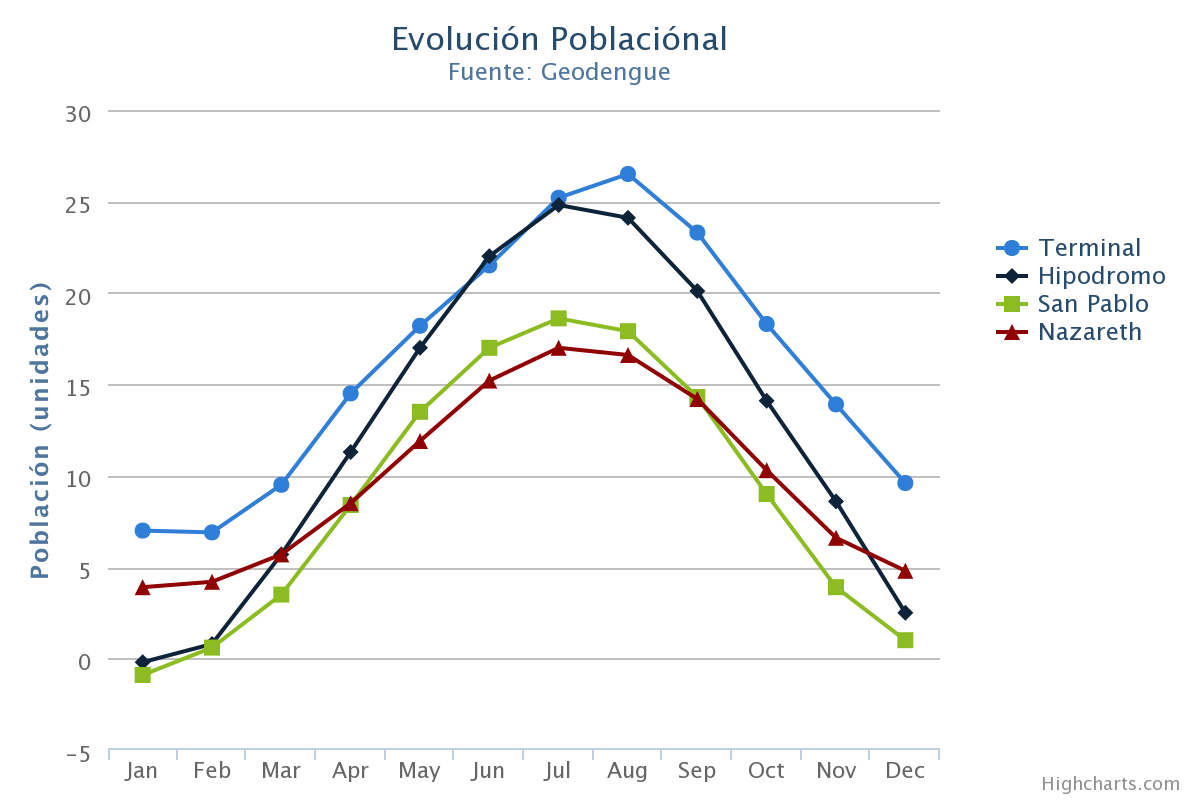
\includegraphics[ scale=0.35]{./graphics/salida-estimada.png}
El proceso de evolución de las muestras consiste en un proceso, en el cual las muestras obtenidas mediante los dispositivos de ovipostura  son expuestas a un conjunto de variaciones en un periodo de tiempo. Las variaciones que, principalmente, afectan a las muestras son
Las variaciones del clima en dicho periodo : Se someten las muestras obtenidas a las distintas variaciones climáticas ocurridas en el periodo de tiempo seleccionado para el estudio.
La naturaleza del mosquito : Cada elemento de la muestra, es sometido a cambios considerando la naturaleza del mosquito. Los aspectos que se tienen en cuenta son su ciclo de vida del mosquito, ciclo reproductivo y el desplazamiento.

\subsection{Cobertura}
*1- Comparar los layers de densidad poblacional con el de focos de dengue, el impacto que puede tener, la posible cantidad de gente a las que puede afectar el foco.
*2- Interpolar nuestras variables utilizando el método adecuado para cada variable, esto es para combinar los layers y buscarle algún significado a la combinación.











%%!TEX root = ../tesis.tex
\chapter{Tecnolog\'ias y Herramientas}
\label{sec:tecnologias}



%figura

% introduccion

%~ aplicaciones



\appendix   % inician los apendices de tu tesis

% los cap'itulos que incluyas a partir de aqu'i aparecen
% como ap'endices

% estos comandos generan la bilbiograf'ia
\printbibliography

\end{document}
